\section{Implementation}
\label{sec:implementation}

The proposed decentralized cloud platform consists of several key components:

\begin{itemize}
    \item \textbf{Nodes and Networking:} The platform runs numerous nodes, and each node adds its resources such as processing power, storage, and bandwidth. The network functions on a divide-and-conquer principle, minimizing communication between different applications running on the network. This strategy enables the network to scale and accommodate numerous nodes and tasks.

    \item \textbf{Reputation System:} The platform uses a blockchain-based system to ensure the security, transparency, and fairness of resource allocation. Smart contracts are utilized to verify that node providers, nodes, and developers are all acting appropriately, and that each party is suitably rewarded for their contributions or penalized for any misconduct.

    \item \textbf{Task Scheduling:} The platform uses a matching engine and, possibly, machine learning algorithms to allocate resources and schedule tasks efficiently. Task scheduling takes into account factors such as task resource requirements, the resources of each node, network conditions, and the reputation of nodes, node providers, and developers. The task scheduling process is designed to be dynamic and adaptive, capable of adjusting to changes in network and task conditions.

    \item \textbf{Token Economics:} The platform employs a distinct dual-token system: one that can be used for transactional purposes and another for reputation tracking. The transactional token facilitates financial interactions between node providers and developers, while the reputation token, non-exchangeable in nature, is earned by node providers and developers during transactions.

    \item \textbf{Application Support:} The platform supports a wide range of applications, from scientific computing and machine learning to web hosting and data storage. The platform provides APIs and SDKs that simplify the process for developers to build and deploy their applications on the platform.
\end{itemize}


\subsection{Nodes and Networking}
\label{sec:nodes_and_networking}

The foundation of the proposed decentralized cloud platform lies in its nodes and the networking infrastructure that connects them. The platform operates on a multitude of nodes, each contributing resources such as processing power, storage, and bandwidth. This section provides a detailed overview of the nodes and networking component of the platform.

\subsubsection{Nodes}
\label{subsec:nodes}

In the context of our platform, a node is a computing device that participates in the network. Each node contributes its computational resources, including processing power (CPU), memory (RAM), storage (hard disk or SSD), and network bandwidth. Nodes can vary in size, from personal computers to large data center servers. This diversity in node capabilities is a strength of the platform, as it allows for a wide range of application requirements.

Each node operates a software client that enables its participation in the network. This client manages the node's resources, communicates with other nodes, and executes assigned tasks. The client software is designed to be lightweight and efficient, minimizing its impact on the node's performance.

\subsubsection{Networking}
\label{subsec:networking}

The networking component of the platform connects nodes and facilitates their communication. The network employs a divide-and-conquer approach, where nodes belonging to a specific developer form a smaller subnetwork or cluster. These clusters maintain direct communication within themselves, and communication between different clusters is minimal unless explicitly established by the developer.

Node providers, who typically host many Nodes or Virtual Machines (VMs), do not need to provide a public IPv4 address for each Node. This is crucial as IPv4 addresses are a scarce resource. Instead, node providers only need to port forward, thereby publicly exposing a few ports for each Node. These ports can be used for peering different nodes of the same developer. For example, some developers may peer nodes with \href{https://nats.io/}{Nats.io}, while others might use \href{https://www.wireguard.com/}{WireGuard}, but any other solution of the developer's choice would work.

Node providers also need to have HTTP and HTTPS ingress, on which a reverse proxy is set up. This reverse proxy forwards requests to the appropriate VM using Server Name Indication (SNI) technology, i.e., based on the target domain name. This routing can be done {\em without} SSL termination to prevent Node providers from being able to snoop all ingress traffic. For this, tools like \href{https://www.haproxy.com/blog/enhanced-ssl-load-balancing-with-server-name-indication-sni-tls-extension}{HAProxy} or recent versions of \href{https://nginx.org/en/docs/stream/ngx_stream_ssl_preread_module.html}{Nginx} can be used. This approach improves security, as it prevents node providers from inspecting traffic to and from nodes.

The illustrated networking approach minimizes communication between nodes in different clusters, reducing network congestion and improving performance.

\begin{figure*}[ht]
    \centering
    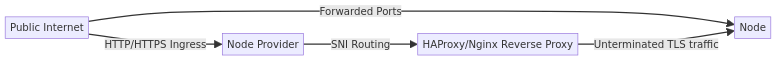
\includegraphics[width=\textwidth]{figures/impl-networking.png}
    \caption{Networking Diagram. Note that blockchain (and the consensus protocol) are not on the data path, so the node performance isn't limited by the consensus speed. Blockchain is on the control path only and is primarily used for tracking reputation.}
    \label{fig:networking_diagram}
\end{figure*}


\subsubsection{Security}

While premium security is a necessity, it often comes with a cost. Techniques such as homomorphic encryption, although secure, can significantly slow down operations and inflate data size by a factor of 10 to 100 or more.

Technologies like Intel SGX and TDX, AMD SEV-SNP, ARM TrustZone, and open-source efforts like UC Berkeley's Keystone offer robust security at a relatively low cost. However, the use of Confidential Computing VMs can lead to a slight performance loss and added complexity. Certain operations are currently unsupported with Confidential Computing VMs:

\begin{enumerate}
    \item Nested virtualization: Running a VM within another VM is not feasible.
    \item Memory overcommitment: Confidential VMs' encrypted memory limits the ability to share or swap out memory, hindering memory overcommitment.
    \item VM snapshots, cloning, and live migration: The hardware-specific encryption keys make it impossible to migrate the encrypted memory state to another host, increasing downtime risk.
    \item Debugging and Inspection: The VM's encrypted and isolated memory state complicates troubleshooting and monitoring.
    \item High-performance Computing (HPC): Direct, low-latency access to hardware resources required by some HPC workloads can be complicated by the additional encryption and isolation layer.
    \item Hardware Compatibility: Not all hardware platforms or devices are compatible with confidential computing technologies.
\end{enumerate}

Despite these challenges, Confidential Computing VMs are invaluable in scenarios where sensitive data needs to be processed or stored securely. These include:

\begin{enumerate}
    \item Private Token Management and Rotation: Confidential computing securely handles sensitive operations like token management and rotation.
    \item SSL Certificate Renewal and Key Storage: Renewing SSL certificates and storing private keys can be securely managed within a confidential computing environment.
    \item Secure Multi-party Computation: Confidential computing provides a secure environment for computation in scenarios where multiple parties need to collaborate on sensitive data.
    \item Data Privacy and Compliance: Confidential computing can help meet strict data privacy and compliance requirements in industries handling sensitive data.
    \item Intellectual Property Protection: Confidential computing ensures that sensitive intellectual property, such as proprietary algorithms or models, are not exposed.
\end{enumerate}

The proposed strategy is to facilitate the use of both regular and Confidential Computing VMs, thereby providing developers with the flexibility to select VM types based on their specific requirements. For example, developers could manage confidential workloads using Confidential Computing VMs, while employing regular VMs for all other workloads. This approach promotes a tailored and efficient use of resources, aligning with the individual needs of each workload.

\subsection{Reputation System}
\label{sec:reputation_system}

The reputation system is the cornerstone of our platform, maintaining simplicity comparable to existing cloud platforms while reliably running conventional workloads on a globally distributed network of node providers. It enhances security, transparency, and fairness in resource allocation. All participants' reputations, including developers and node providers, are tracked via smart contracts on a blockchain.

When a developer pays a node provider, the system charges the node provider a 2\% fee. A portion of this fee is automatically transferred to a DAO-controlled wallet that finances research and development efforts. In return, the reputations of both the developer and the node provider increase by 1\%.

Assuming mostly honest behavior, the reputations of developers and node providers will gradually grow, proportional to the service payment amounts and transactions performed on the platform. All reputations are publicly visible, allowing, but not forcing, node providers and developers to restrict their interactions to high-reputation parties. Additionally, node providers' reputations are used to reward them for offering nodes for rent, making it crucial for all node providers to maintain a high reputation.

If either a node provider or a developer is dissatisfied with the service or collaboration, they can spend their reputation to reduce the other's reputation. The sender's reputation decreases by the amount spent, while the receiver's reputation decreases by a higher amount, such as 200\%, to incentivize honest and cooperative behavior. For members with high reputations, these reductions can be severe in extreme cases. Spending hard-earned reputation to reduce another party's reputation is not undertaken lightly, as rebuilding reputation takes significant time and money.

Reputation is hard to earn and easy to lose, encouraging all parties to uphold high standards of quality, communication, and integrity at all times, while still offering a means to penalize potentially dishonest or malicious behavior, in a general and transparent manner.

\begin{figure}[ht]
    \centering
    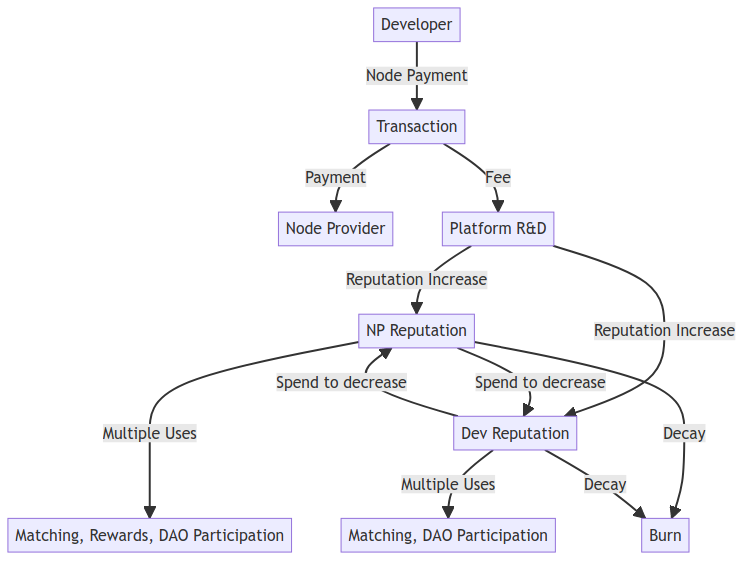
\includegraphics[width=\columnwidth]{figures/impl-reputation.png}
    \caption{Reputation tracking system, running on Blockchain.}
    \label{fig:reputation-system}
\end{figure}


\subsection{Resource Allocation}
\label{sec:resource_allocation}

The platform employs a matching engine and, if necessary, machine learning algorithms to efficiently allocate resources and match developers with suitable nodes.

A developer specifies their requirements, which may include some or all of the following:
\begin{itemize}
    \item Acceptable price
    \item Required virtual CPU (vCPU)
    \item Required Random Access Memory (RAM)
    \item Required storage (which can be unlimited)
    \item Required network bandwidth (which can be unlimited)
    \item Minimum node provider reputation
    \item Renting period
\end{itemize}

The matching engine processes these requirements and returns a list of suitable nodes. The developer then selects one or more nodes from this list and sends a request to confirm the rental. Upon receiving payment from the developer, the matching engine provides a rental contract ID. The developer can use this contract ID to start utilizing the node.

If the developer wishes to extend the rental period, they can make another request at a later time. The process for extending the rental period is similar to the original rental process, with the key difference being that the developer already has access to the node.


\subsection{Token Economics (Tokenomics)}
\label{sec:token_economics}

The platform tokenomics balances two key components: (1) the Decentralized Cloud Token (DCT), with which all key platform operations are paid, and (2) the actor reputation, which is hard to earn and easy to lose. The reputation is discussed in more details in Section~\ref{sec:reputation_system}.

{\bf Token Minting (Generation) and Distribution.}
Similar to Bitcoin, DC tokens are minted in each new block, occurring approximately every 10 minutes. The initial block mints 50 tokens, and after that the minted tokens are halving every 210,000 blocks. This model is designed to sustain token supply growth at a decreasing rate, with a final cap due to the smallest unit set by the DC token's nine decimal places, calculated to total of approximately 21,000,000 DC tokens.

The distribution of DC tokens received in a block are weighted by their reputation within the protocol. This reputation is dynamically adjusted based on participants' transaction activities and behaviors. The reward distribution uses a square root scaling function to calculate weights, providing diminishing returns on increased reputation scores, thereby maintaining incentives for both high and low-reputation participants.

Importantly, there will be no other DCT generation other than through this minting and rewarding process. There will be no additional token sale, airdrop, or any other form of token distribution. This approach promotes fair distribution of DCT across participants and balances supply and demand over time.

{\bf Project Funding.}
Participation in the DC token reward distribution requires a fee, set at 1/100th of the block reward, creating a steady funding stream for project-related activities. These fees are directed to predetermined wallets, which include known wallets designated for project development. This ensures transparency in funding flows and supports ongoing development efforts.

{\bf Stability, Governance, and Community Engagement.}
The stability and security of the token value are ensured through several mechanisms. Firstly, the supply of DCT is both limited and predictable, which, when balanced against the inherent demand created by developers needing to rent nodes, aids in maintaining market equilibrium. Secondly, the platform's Decentralized Autonomous Organization (DAO) has the capability to implement necessary adjustments to the reward system. This flexibility allows for the mitigation of extreme price volatility. Finally, the platform is committed to adhering to all relevant legal and regulatory standards, further ensuring the security of transactions and the integrity of the token system.

This model would facilitate community input through a transparent proposal system where community members can submit and vote on changes. It will also be possible to implement a delegated governance model, to address potential voter apathy and ensure informed decision-making.

{\bf Token Demand and Supply.}
Developers and node providers need to obtain DCT in order to pay for the registration fee. The DCT token can be obtained on an exchange, and the exchange obtains the token from one of the existing token holders. This creates an inherent demand for DCT. Node providers, on the other hand, will need to cover costs such as electricity and internet connectivity, which may necessitate selling a portion of their DCT. However, some providers may choose to retain a portion of their DCT in anticipation of a price increase, which could, in turn, increase the likelihood of such a price increase and creating a virtuous circle.

{\bf Smart Contract Interoperability.}
The system would run on the Internet Computer platform and DCT would adhere to the ICRC-1 and potentially also newer token standard to ensure compatibility and ease of integration with wallets and exchanges. In the future, an exploration of cross-chain functionality will take place, to enhance liquidity and utility across different blockchain ecosystems.

\subsection{Application Support}
\label{sec:application_support}

The ability to support a wide range of applications is a critical factor for the success of any computing platform. This versatility not only broadens the platform's potential user base but also increases its utility and value for each user. By accommodating various types of applications, from scientific computing and machine learning to web hosting and data storage, the platform can cater to diverse needs and use cases, thereby attracting a wider audience and fostering a vibrant and diverse user community \cite{gawer2002platform}.

Our platform is designed with this versatility in mind. It provides comprehensive support for a wide range of applications, enabling developers to leverage the platform's resources and capabilities to build and deploy various types of applications. This is in line with the best practices in platform design, which emphasize the importance of flexibility and extensibility in supporting diverse applications \cite{meyer1997power}.

To facilitate application development and deployment, the platform provides Application Programming Interfaces (APIs) and Software Development Kits (SDKs). These tools simplify the process for developers to interact with the platform, abstracting away the complexities of the underlying infrastructure. This aligns with the principles of developer experience, which highlight the importance of providing developers with effective tools and resources to enhance their productivity and satisfaction \cite{ko2006exploratory}.

Moreover, the platform is designed to be permissionless, meaning that the community of node providers and developers themselves can decide what kind of support should be added. For instance, there is nothing stopping node providers from adding nodes with GPU support, even though this is not something that is explicitly supported or required by the platform. This permissionless nature fosters innovation and allows the platform to adapt to the evolving needs of its community.

In conclusion, by providing comprehensive application support, continuously adapting to the evolving needs of developers, and allowing the community to drive innovation and expansion, our platform aims to be a versatile and valuable tool for a wide range of applications.
